

\tikzset{every picture/.style={line width=0.75pt}} %set default line width to 0.75pt        

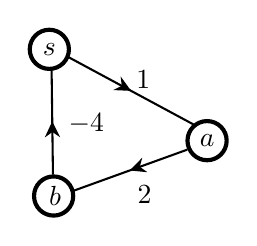
\begin{tikzpicture}[x=0.5pt,y=0.5pt,yscale=-1,xscale=1]
%uncomment if require: \path (0,174); %set diagram left start at 0, and has height of 174

%Straight Lines [id:da6034488908673977] 
\draw [color={rgb, 255:red, 0; green, 0; blue, 0 }  ,draw opacity=1 ][line width=0.75]    (146,105) -- (63,135) ;
\draw [shift={(104.5,120)}, rotate = 340.13] [fill={rgb, 255:red, 0; green, 0; blue, 0 }  ,fill opacity=1 ][line width=0.08]  [draw opacity=0] (11.61,-5.58) -- (0,0) -- (11.61,5.58) -- (7.71,0) -- cycle    ;
%Straight Lines [id:da5375746664082175] 
\draw [color={rgb, 255:red, 0; green, 0; blue, 0 }  ,draw opacity=1 ][line width=0.75]    (151,87) -- (60,38) ;
\draw [shift={(105.5,62.5)}, rotate = 208.3] [fill={rgb, 255:red, 0; green, 0; blue, 0 }  ,fill opacity=1 ][line width=0.08]  [draw opacity=0] (11.61,-5.58) -- (0,0) -- (11.61,5.58) -- (7.71,0) -- cycle    ;
%Straight Lines [id:da43457397683408727] 
\draw [color={rgb, 255:red, 0; green, 0; blue, 0 }  ,draw opacity=1 ][line width=0.75]    (48,46) -- (49,123) ;
\draw [shift={(48.5,84.5)}, rotate = 89.26] [fill={rgb, 255:red, 0; green, 0; blue, 0 }  ,fill opacity=1 ][line width=0.08]  [draw opacity=0] (11.61,-5.58) -- (0,0) -- (11.61,5.58) -- (7.71,0) -- cycle    ;

% Text Node
\draw  [line width=1.5]   (46.38, 32.47) circle [x radius= 14.15, y radius= 14.15]   ;
\draw (46.38,32.47) node   [align=left] {$\displaystyle s$};
% Text Node
\draw  [line width=1.5]   (49.48, 138.47) circle [x radius= 14.15, y radius= 14.15]   ;
\draw (43.98,138.47) node [anchor=west] [inner sep=0.75pt]   [align=left] {$\displaystyle b$};
% Text Node
\draw  [line width=1.5]   (160.38, 98.47) circle [x radius= 14.15, y radius= 14.15]   ;
\draw (160.38,98.47) node   [align=left] {$\displaystyle a$};
% Text Node
\draw (107,45.47) node [anchor=north west][inner sep=0.75pt]   [align=left] {$\displaystyle 1$};
% Text Node
\draw (108,128.47) node [anchor=north west][inner sep=0.75pt]   [align=left] {$\displaystyle 2$};
% Text Node
\draw (58,76.47) node [anchor=north west][inner sep=0.75pt]   [align=left] {$\displaystyle -4$};


\end{tikzpicture}

